\documentclass[12pt]{article}
\usepackage{baseset}
\usepackage{myproblem}
\usepackage{stackengine}
\DeclareSymbolFont{operators}{OT1}{ntxtlf}{m}{n}
\SetSymbolFont{operators}{bold}{OT1}{ntxtlf}{b}{n}
\usepackage{wasysym}
\newcommand{\RomanNumeralCaps}[1]
{\MakeUppercase{\romannumeral #1}}
\usepackage{tabularx}
\usepackage{enumitem}

\begin{document}
\begin{tabularx}{\textwidth}{Xr}
{\Large \textbf{Праки}} & Взлёт $27.11.2023$ \\
\end{tabularx}
\noindent\rule{\textwidth}{0.4pt}
\begin{enumerate}
    \item На рисунке представлена кривая блеска двойной звезды, полученная в фильтре $V$. Зная, что затмения в системе центральные, один из компонентов двойной имеет спектральный класс $A0$, а второй - $G2$, и оба компонента являются звёздами главной последовательности, постройте кривую изменения показателя цвета $B - V$ этой системы. Ось ординат Вашего графика направьте вверх, нанесите деления и поставьте соответствующие значения показателей цвета. \\

    \begin{figure}[h]
        \centering
        \begin{tikzpicture}
            \begin{axis}[
                xlabel = {время $t$, условные единицы},
                ylabel = {$V_{\Sigma}$, блеск в фильтре $V$},
                minor tick num = 2,
                y dir=reverse,
                height = 0.28\paperheight, 
                width = 0.6\paperwidth,
                xtick={-5, 0,...,25},
                grid=major
            ]
            \addplot[thick, black, mark=none] coordinates {(-2.75, 9.98) (-2.25, 9.98) (-1.5, 10.1) (1.5, 10.1) (2.25, 9.98) (8.75, 9.98) (10, 10.0) (12.75, 10.0) (14.0, 9.98) (20.0, 9.98) (20.75, 10.1) (23.75, 10.1) (24.5, 9.98) (25, 9.98)};
            \end{axis}
        \end{tikzpicture}
    \end{figure}

    \item Вам дана зависимость высоты некоторой звезды от её астрономического азимута. Определите широту места наблюдение и склонение звезды.
    \begin{figure}[h]
        \centering
        \begin{tikzpicture}
            \begin{axis}[
                table/col sep = comma,
                height = 0.28\paperheight, 
                width = 0.6\paperwidth,
                minor tick num = 4,
                ylabel = {$h,^\circ$},
                xlabel = {$A,^\circ$},
                only marks,
                mark size = 1 pt
                ]
                \addplot[black, mark = *] table [y={h}, x={A}] {ha.csv};
            \end{axis}
        \end{tikzpicture}
    \end{figure}
    \newpage
    \item На графике представлено распределение энергии в спектре одной из звезд,
    окружённой пылевой оболочкой. Известно, что оболочка состоит из чернотельных пылинок, она сферически симметричная и геометрически тонкая (т.е. её толщиной можно пренебречь по сравнению с радиусом). Параллакс звезды $0.002"$. Определите радиус центральной звезды, если известно,
    что её эффективная температура $7~000$ K. Чему равна температура пылинок
    и оптическая толща пылевой оболочки в видимом диапазоне длин волн?
    \begin{figure}[h]
        \center{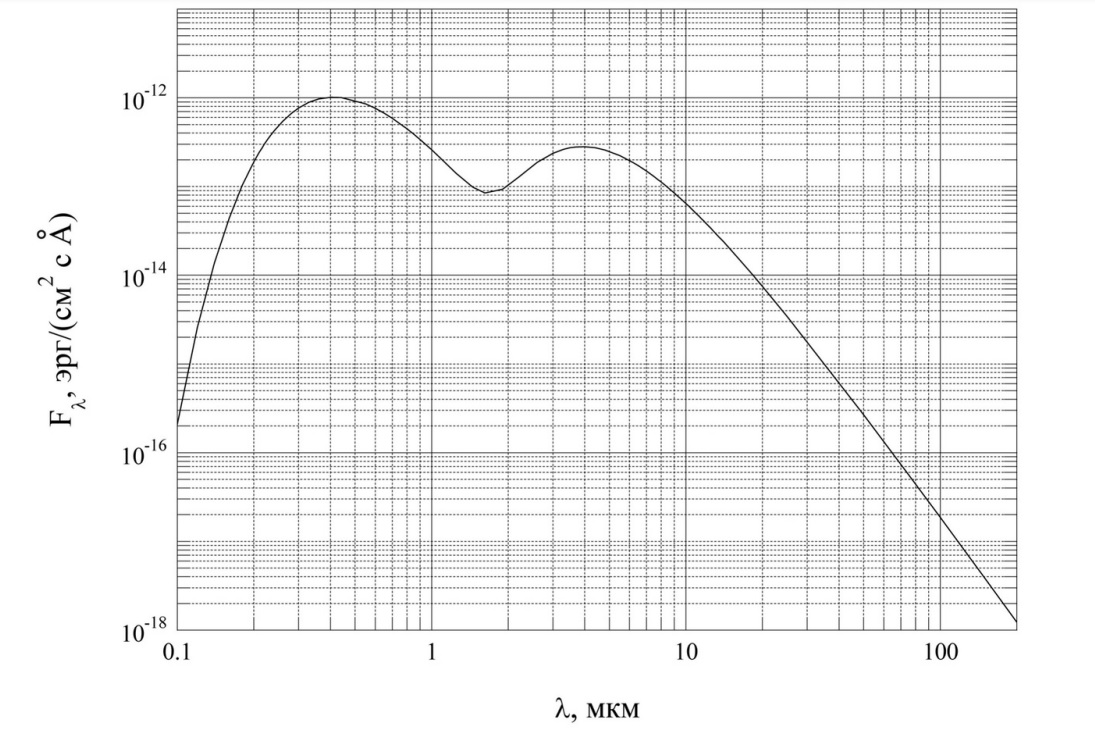
\includegraphics[width = \linewidth]{spectr1.jpg}}
    \end{figure}
    
    \newpage
    \item При обработке наблюдений галактик в ранней Вселенной была обнаружена галактика, похожая на Млечный Путь ($М_b = -21^m$, $D = 30$ кпк). Измеренная её болометрическая звёздная величина составила $27.8^m$, а угловой размер -- $5.3''$. Определите по этим данным красное смещение найденной галактики и сопутствующее расстояние до неё.
    В этом Вам может помочь приведённый график, на котором изображены зависимости фотометрического (по наблюдаемой яркости), углового (по наблюдаемому угловому размеру) и сопутствующего (геометрического на момент наблюдения) расстояния для нашей вселенной. Но, к сожалению, информация о том, какая кривая соответствует какому расстоянию, оказалась утеряна.
    Нарисуйте на графике в бланке ответа кривую, соответствующую расстоянию, получаемому из классического закона Хаббла и классического эффекта Доплера.
    \begin{figure}[h]
        \center{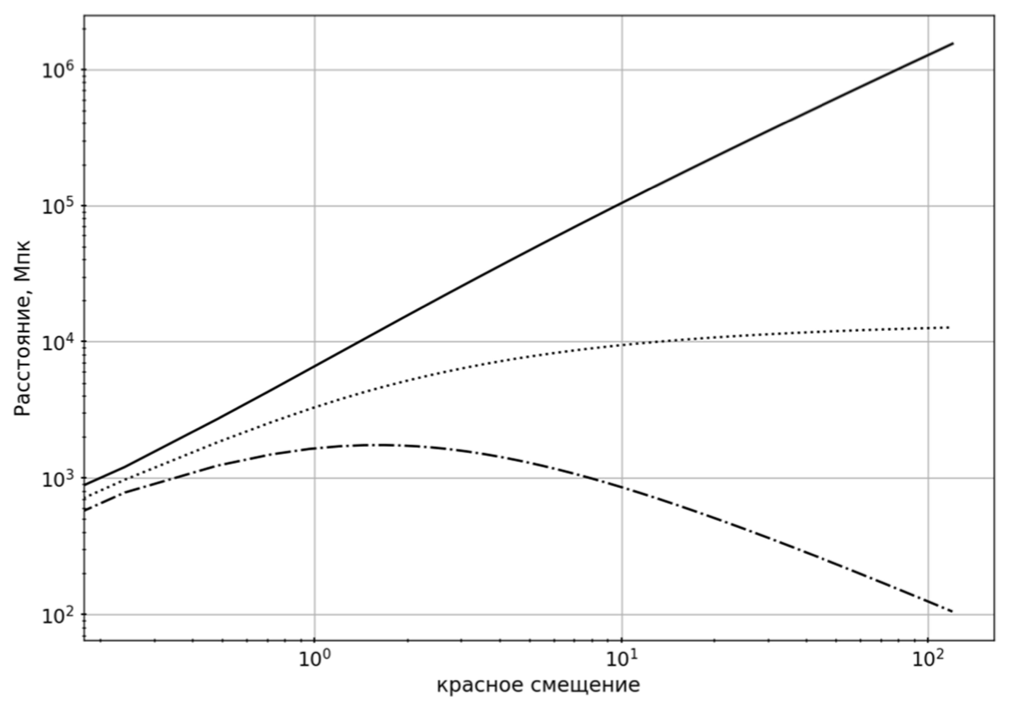
\includegraphics[width = \linewidth]{img7.png}}
    \end{figure}
\end{enumerate}
\end{document}